\documentclass[tikz]{standalone}

% tikz picture of a flash drum with heat exchanger and pressure
% reducing valve.

\usepackage[scaled]{helvet}
\renewcommand\familydefault{\sfdefault} 
\usepackage[T1]{fontenc}

\usepackage{sansmath}
\begin{document}

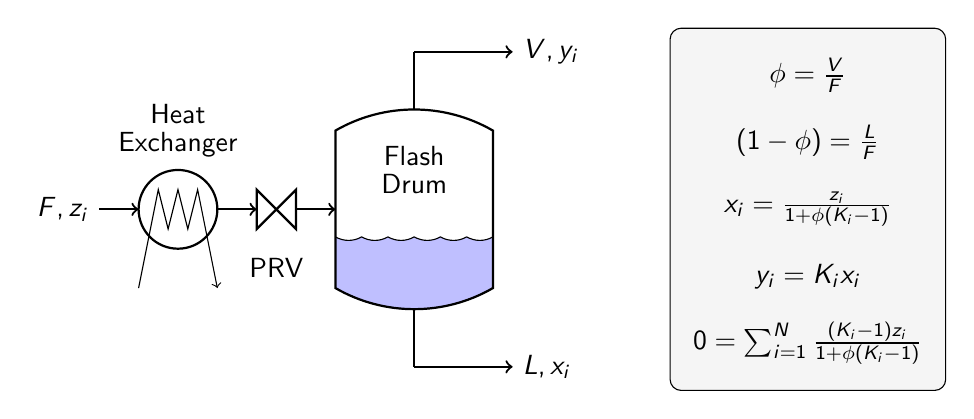
\begin{tikzpicture}
\begin{sansmath}
  %\draw[step=1cm,gray,very thin] (0,0) grid (12,6);
  
  % Coordinates
  \coordinate (drum) at (4,3);
  \coordinate (feed) at (1,3);
  \coordinate (hx) at (1.5,3);
  \coordinate (valve) at (3,3);
  \coordinate (eqns) at (10,3);

  % Drum outline. Given location of the feed port, draws a drum with
  % stubs for the liquid and vapor lines located at ++(1,2) and ++(1,-2)
  \draw[fill=blue!25] (drum) ++(0,-1) arc (240:300:2cm) -- ++(0,0.65)
    arc(-60:-120:0.333cm) arc(-60:-120:0.334cm) arc(-60:-120:0.333cm) 
    arc(-60:-120:0.333cm) arc(-60:-120:0.334cm) arc(-60:-120:0.333cm);
  \draw[thick] (drum) --++(0,-1) arc (240:300:2cm)
    -- ++(0,2) arc (60:120:2cm) -- ++(0,-1);
  \draw[thick] (drum) ++(1,1.268) -- ++(0,0.732); 
  \draw[thick] (drum) ++(1,-1.268) --++ (0,-0.732);
    
  % Heat Exchanger. Given location of the feed port, draws an exchanger
  % with outlet at ++(1,0) and coolant ports at ++(0,-1) and ++(1,-1).
  \draw[thick] (hx) arc(+180:-180:0.5cm);
  \draw [->] (hx) ++(0,-1) -- ++ (0.25,1.25) -- ++(0.125,-0.5) -- ++(0.125,0.5)
    -- ++(0.125,-0.5) -- ++(0.125,0.5) -- ++(0.25,-1.25);

  % Pressure reducing value. Given location of the feed port, draws a
  % a valve with outlet at ++(0.5,0)
  \draw [thick] (valve) -- ++(0,0.25) -- ++(0.5,-0.5)
    -- ++(0,0.5) -- ++(-0.5,-0.5) --++(0,0.25);
  
  % connecting the units
  \draw[->,thick] (feed) node [left] {$F, z_i$} -- (hx);
  \draw[->,thick] (hx) ++ (1,0) -- (valve);
  \draw[->,thick] (valve) ++ (0.5,0) -- (drum);
  \draw[->,thick] (drum) ++ (1,2) -- ++(1.25,0) node [right] {$V, y_i$};
  \draw[->,thick] (drum) ++ (1,-2) -- ++(1.25,0) node [right] {$L, x_i$};
  
  % label units
  \draw (hx) ++ (0.5,1) node {\shortstack{Heat \\ Exchanger}};
  \draw (valve) ++ (0.25,-0.75) node {PRV};
  \draw (drum) ++ (1,0.5) node {\shortstack{Flash \\ Drum}};
  
  % equations
  \draw[rounded corners,fill=gray!8] (eqns) +(-1.75,-2.3) rectangle +(1.75,2.3);
  \draw (eqns) 
    +(0,1.7) node {$\phi = \frac{V}{F}$}
    +(0,0.85) node {$(1-\phi) = \frac{L}{F}$}
    +(0,0) node {$x_i = \frac{z_i}{1+\phi(K_i-1)}$}
    +(0,-0.85) node {$y_i = K_i x_i$}
    +(0,-1.7) node {$0 = \sum_{i=1}^N \frac{(K_i-1)z_i}{1+\phi(K_i-1)}$};
\end{sansmath}
\end{tikzpicture}
\end{document}